\chapter{Logica}
Come già visto più volte, i linguaggi possono essere rappresentati in modi differenti, tramite modelli e astrazioni via via più potenti, tra cui:
\begin{itemize}
  \item Insiemi;
  \item Pattern;
  \item Espressioni Regolari;
  \item Modelli Operazionali (come gli Automi);
  \item Modelli Generativi (come le Grammatiche);
  \item Modelli Dichiarativi (come la Logica).
\end{itemize}

\noindent
I concetti di logica introdotti di seguito sono utilizzati per definire in maniera differente i linguaggi.

\section{Logica Proposizionale}
Il calcolo proposizionale, detto anche logica proposizionale, è un modello dichiarativo formale della logica matematica che si basa sul concetto di proposizione, ovvero frasi che possono assumere solamente il valore vero o il valore falso. In generale, ogni linguaggio consiste di una sintassi e di una semantica: la sintassi è l'insieme delle regole attraverso cui è possibile costruire le frasi di cui il linguaggio è composto, mentre la semantica spiega il significato delle varie frasi del linguaggio. 

\paragraph*{Sintassi}
In modo formale:
\begin{definition}
  La logica proprosizionale è composta da un linguaggio \(\mathcal L\), il cui alfabeto è costituito dai seguenti elementi:
  \begin{enumerate}
    \item Un insieme numerabile (finito o non) di proposizioni (simboli di relazione nullaria), che possono essere simboli, stringhe o frasi;
    \item Un insieme di connettivi logici: \(\lnot\) (NOT), \(\wedge\) (AND), \(\vee\) (OR), \(\Rightarrow\) (Implicazione) e \(\Leftrightarrow \)(Coimplicazione);
    \item Un insieme di simboli di punteggiatura: ( e )
  \end{enumerate}
  I simboli che compongono l'alfabeto sono privi di significato: assegnarne uno è compito della semantica. 
\end{definition}

\begin{table}[!th] \label{Tabella delle verità}
  \caption{Tabella della verità dei connettivi logici}
  \vspace*{10pt}

  \centering
  \begin{tabular}{c c || c | c | c | c | c }
    \(F\) & \(G\) & \(\lnot F\) & \(F \wedge G\) & \(F \vee G\) & \(F \Rightarrow G\) & \(F\Leftrightarrow G\) \\
    \hline
    T & T & F & T & T & T & T \\
    T & F & F & F & T & F & F \\
    F & T & T & F & T & T & F \\
    F & F & T & F & F & T & T \\
  \end{tabular}  
\end{table}

Una proposizione si dice essere atomica quando non può essere scomposta in parti più piccole. Nel caso contrario, la proposizione è composta da due o più proposizioni più piccole legate fra loro tramite i connettivi logici appena introdotti. Le parentesi sono utilizzare per modificare la precedenza dei connettivi, che di base avrebbero il seguente ordine logico: \(\lnot, \wedge, \vee, \Rightarrow, \Leftrightarrow\).

La sintassi del linguaggio definisce le sequenze ammissibili di simboli sull'alfabeto, le cosiddette formule ben formate (fbf). L'insieme di queste formule ben definite su \(\mathcal L\) è il più piccolo insieme tale che ogni proposizione è una formula e, se \(F\) e \(G\) sono formule, allora anche \(\lnot F\), \(F \wedge G\), \(F \vee G\), \(F \Rightarrow G\) \(F \Leftrightarrow G\) sono formule. In logica proposizionale si ha che se \(A\) è una proposizione, allora \(A\) e \(\lnot A\) sono letterali, in cui \(A\) è letterale positivo, mentre \(\lnot A\) è letterale negativo. Infine, si dice letterale complementare la proposizione \(\bar L\) definito come \(\lnot A\) se \(L=A\), oppure \(A\) se \(L=\lnot A\). 

\break

Una volta introdotte le formule ben formate, è possibile definire le sottoformule, ovvero una parte di una fbf che è a sua volta una fbf. L'insieme  \(Stfm(F)\) delle sottoformule di \(F\) è definito come il più piccolo insieme di formule tale che:
\begin{itemize}
  \item \(F \in Stfm(F)\);
  \item Se \(\lnot G \in Stfm(F)\), allora \(G \in Stfm(F)\);
  \item se \(G \wedge H, G\vee H, G \Rightarrow H, G \Leftrightarrow H \in Stfm(F)\), allora \(H, G \in Stfm(F)\). 
\end{itemize}

\paragraph*{Semantica}
La semantica, invece, ha lo scopo di assegnare un significato alle formule appena definite, tramite una funzione \(I\), detta interpretazione, che mappa ogni proposizione ad un valore di verità (vero o falso): formalmente, \(I: \{fbf\} \to \{0,1\}\). Tale funzione, quindi, non fa altro che assegnare il valore di vero (1) o falso (0) alle lettere proposizionali costanti \footnote{Le lettere proposizionali costanti sono \(T\) (o \(V\)) per rappresentare una proposizione vera, oppure \(\bot\) (o \(F\)) per rappresentare una proposizione falsa} e valuta il valore di verità di \(\lnot F, F \wedge G, F \vee G, F \Rightarrow G, F \Leftrightarrow G\) sulla base dei valori di verità delle proposizioni \(F\) e \(G\). 

Da qui, si introduce il simbolo \(\vDash\) (doppio tornello), che si utilizza per associare formule ed interpretazioni. Dunque, la scrittura \(I \vDash F\), che si legge \(I\) rende vera \(F\), vale nei seguenti casi:
\begin{itemize}
  \item \(I \vDash A\) se e solo se \(I(A) = T\), con \(A\) proposizione;
  \item \(I \vDash \lnot F\) se e solo se \(I \nvDash F\);
  \item \(I \vDash F \wedge G\) se e solo se \(I\vDash F\) e \(I \vDash G\);
  \item \(I \vDash F \vee G\) se e solo se \(I \vDash F\) o \(I \vDash G\);
  \item \(I \vDash F \Rightarrow G\) se e solo se \(I \nvDash G\) o \(I \vDash G\);
  \item \(I \vDash F \Leftrightarrow G\) se e solo se \(I \vDash F\Rightarrow G\) e \(I \vDash G \rightarrow F\).
\end{itemize}

\noindent
Dal concetto di interpretazione, si possono definire le seguenti proprietà della semantica delle formule proposizionali:
\begin{itemize}
  \item Se \(I\vDash F \), allora si dice che \(I\) è un modello di \(F\);
  \item \(F\) si dice valida (o si dice essere una tautologia) se e solo se per ogni interpretazione \(I\) vale che \(I \vDash F\);
  \item \(F\) è soddisfacibile se e solo se esiste un'interpretazione \(I\) tale che \(I \vDash F\);
  \item \(F\) è falsificabile se e solo se esiste un'interpretazione \(I\) tale che \(I \nvDash F\);
  \item \(F\) è insoddisfacibile se e solo se per ogni interpretazione \(I\) vale che \(I \nvDash F\);
  \item \(F\) è contingente se e solo se è sia soddisfacibile che falsificabile;
  \item Ogni formula del tipo \(F \wedge \lnot F\) è una contraddizione, indicata con \(\bot\);
  \item Ogni formula del tipo \(F \vee \lnot F\) è detta principio del terzo escluso, indicata con \(\top \)
\end{itemize}

\paragraph{}
Un insieme di formule \(\mathcal F\) comporta logicamente una formula \(G\) o, equivalentemente, una formula \(G\) è una conseguenza logica di un insieme di formule \(\mathcal F\), se ogni modello di \(\mathcal F\) è anche un modello di \(G\) e si scrive con \(\mathcal F \vDash G\). Dopo aver stabilito una corrispondenza semantica fra due formule logiche, è possibile anche stabilire una relazione di equivalenza fra due formule logiche, relazione che vale solamente se la corrispondenza fra le due formule è biunivoca, ovvero se vale sia \(F \vDash G\) che \(G \vDash F\): una tale relazione si rappresenta con la scrittura \(F \equiv G\).

Esistono innumerevoli equivalenze notevoli:
  \begin{flalign*}
    F \wedge F &\equiv F \\
    F \vee F &\equiv F \\
    F \wedge G &\equiv G\wedge F \\
    F \vee G &\equiv G \vee F \\
    F \wedge (G \wedge H) &\equiv (F \wedge G) \wedge H\\
    F \vee (G \vee H) &\equiv (F \vee G) \vee H \\
    (F \wedge G) \vee F &\equiv F \\
    (F \vee G) \wedge F &\equiv F \\
    F \wedge (G \vee H) &\equiv (F\wedge G) \vee (F\wedge H) \\
    F \vee (G \wedge H) &\equiv (F \vee G) \wedge (F \vee H) \\
    \lnot\lnot F &\equiv F \\
    \lnot (F\wedge G) &\equiv \lnot F \wedge \lnot G\\
    \lnot (F \vee G) &\equiv \lnot F \wedge \lnot G \\
    F \Leftrightarrow G &\equiv (F \Rightarrow G) \wedge (G \Rightarrow F) \\
    F \Rightarrow G &\equiv \lnot F \vee G \\
    F \Rightarrow G &\equiv \lnot G \Rightarrow  \lnot F
  \end{flalign*}  
In logica prposizionale è anche possibile sostituire una sottoformula \(G\), di una formula ben formata \(F\), con una formula \(H\): la formula risultate viene indicata con la scrittura \(F[G \backslash H]\). Tale sostituzione, però, può avvenire solamente se \(G \equiv H\). 

In base a questi concetti si può notare che non tutti i connettivi logici sono strettamente necessari, in quanto possono essere sostituiti con altri. A questo proposito, un insieme di connettivi è detto funzionalmente completo se e solo se qualunque formula proposizionale può essere trasformata in una formula semanticamente equivalente che contiene solamente i connettivi dell'insieme dato. Sfruttando tali insiemi, detti minimali, e le equivalenze semantiche, è possibile definire delle forme normali, che introducono degli schemi sintattici di completa generalità semantica per scrivere formule, permettendo così di formalizzare il significato di qualsiasi formula che si possa scrivere con la completa generalità della logica proposizionale. In altre parole, per ogni formula ben formata esistono una o più formule logicamente equivalenti ad essa scritte in una forma normale. Esistono tre principali forme normali per la logica proposizionale, chiamate forma negativa, forma congiuntiva e forma disgiuntiva. Una formula è in forma normale negativa se e solo se è composta solamente da letterali, congiunzioni e disgiunzioni; una formula è in forma normale congiuntiva (detta anche CNF) se e solo se ha la forma \(C_1 \wedge C_2 \wedge ... \wedge C_n\), dove \(C_i\) è una disgiunzione di letterali; una formula è in forma normale disgiuntiva (detta anche DFN) se e solo se ha la forma \(D_1 \vee D_2 \vee ... \vee D_n\), dove \(D_i\) è una congiunzione di letterali. 

A questo punto è possibile completare la definizione della logica proposizionale attraverso i concetti di assioma e regole di inferenza, che costituiscono un sistema formale assiomatico-deduttivo (in inglese calculus). Questi elementi definiscono una relazione di derivabilità (relazione già analizzata nel contesto delle grammatiche), detta anche dimostrabilità, tra un insieme di formule \(\mathcal F\) e una formula \(G\). Dunque, i sistemi formali della logica hanno un compito molto simile a quello assolto dalle grammatiche, ovvero producono meccanicamente una formula risultante a partire da un insieme iniziale di formule, applicando assiomi e regole di inferenza. Si scrive, quindi, \(\mathcal F \vdash G\) se \(G\) può essere ottenuto da \(\mathcal F\). Idealmente, la relazione di derivabilità dovrebbe essere corretta (cioè se \(\mathcal F \vdash G\) allora \(\mathcal F \vDash G\)) e completa (cioè se \(\mathcal F\vDash G\) allora \(\mathcal F\vdash G\)). Se una formula \(F\) può essere derivata in una teoria \(\mathcal F\) usando solamente assiomi e regole di inferenza di un sistema, allora si dice che \(F\) è un teorema. 

\section{Logica del Primo Ordine}
La logica proposizionale appena analizzata ha molte applicazioni, ma il suo potere espressivo è ristretto. Per questo motivo, nel 1979 è stata sviluppata  la logica del primo ordine, che permette dal punto di vista ontologico di considerare non solo fatti (come avveniva nella logica proposizionale), ma anche proprietà, relazioni e funzioni. 

\paragraph*{Sintassi}
In modo formale:
\begin{definition}
  La logica del primo ordine è composta da un linguaggio \(\mathcal L\), il cui alfabeto è costituito dai seguenti elementi:
  \begin{enumerate}
    \item Un insieme numerabile infinito di variabili;
    \item Un insieme di simboli di funzione;
    \item Un insieme di simboli di predicati (o relazioni);
    \item Un insieme di connettivi logici: \(\lnot\) (NOT), \(\wedge\) (AND), \(\vee\) (OR), \(\Rightarrow\) (Implicazione) e \(\Leftrightarrow \)(Coimplicazione);
    \item Un insieme di quantificatori: \(\exists\) (Esiste) e \(\forall\) (Per ogni);
    \item Un insieme di simboli di punteggiatura: ( , ) e le virgole.
  \end{enumerate}
  Ogni simbolo di funzione e relazione ha una arietà fissata, che indica il numero di argomenti associati a quella determinata funzione. Le funzioni nullarie sono dette costanti, mentre i predicati costanti sono detti proposizioni. I simboli dell'alfabeto sono privi di significato: assegnarne uno è compito della semantica.
\end{definition}

Per poter scrivere formule nella logica del primo ordine c'è la necessità di denotare tutti gli oggetti di cui il linguaggio \(\mathcal L\) può parlare, detti termini. Tale denotazione avviene induttivamente come segue:
\begin{itemize}
  \item ogni variabile è un termine della formula;
  \item se \(f\) è un simbolo di funzione \(n\)-aria e \(t_1, t_2, ..., t_n\) sono termini, allora \(f(t_1, t_2,...,t_n)\) è un termine.
\end{itemize}

Gli oggetti appena denotati attraverso i termini, si possono utilizzare all'interno delle formule della logica del primo ordine, definite anch'esse in maniera induttiva. L'insieme delle formule della logica del primo ordine è definito come il più piccolo insieme tale che:
\begin{itemize}
  \item Se \(p\) è un simbolo di relazione \(n\)-aria e \(t_1, t_2,...,t_n\) sono termini, allora \(p(t_1, t_2,...,t_n)\) è una formula detta atomica o semplicemente atomo;
  \item Se \(F\) e \(G\) sono formule e \(X\) è una variabile, allora \(\lnot F, F\vee G, F\wedge G, F \Rightarrow G, F \Leftrightarrow G, \exists XF, \forall XF\) sono formule.
\end{itemize}

Nella scrittura di formule appartenenti alla logica del primo ordine, c'è un'osservazione da fare: quando si utilizza il quantificatore \(\forall\) il connettivo principale utilizzato è \(\Rightarrow\), mentre nel caso si utilizzi il quantificatore \(\exists\) allora il connettivo principale è \(\wedge\). Inoltre, se \(QX(F)\) rappresenta una formula in cui \(Q\) è un quantificatre, allora \(F\) si dice ambito di \(Q\) e che \(Q\) è applicato ad \(F\). Un'occorrenza di una variabile in una formula è legata se e solo se la sua occorrenza è entro l'ambito di un quantificatore che impiega quella variabile, altrimenti è libera. Una formula è chiusa se e solo se non contiene occorrenze libere di variabili. Le formule chiuse sono quelle per le quali, data un'interpretazione \(I\), si può calcolare la veridicità.

\paragraph*{Semantica}
Come per il caso della logica proposizionale, anche la logica del primo ordine ha una semantica basata sul concetto di interpretazione: un'interpretazione \(I\) di un alfabeto \(A\) è un dominio non vuoto \(D\) (indicato anche con \(|I|\)) e una funzione che che associa ogni costante \(c\in A\) a un oggetto \(c_I \in D\), ogni simbolo \(n\)-ario di funzione \(f\in A\) a una funzione \(f_I:D^n\to D\) e ogni simbolo \(n\)-ario di predicato \(p\in A\) a una relazione \(p_I\subseteq D\times D\times ... \times D\), \(n\) volte. Prima di poter assegnare un significato alle fromule, va definito il significato di ogni termine, indicato con \(\phi_I(t)\) con \(t\) il termine a cui dare singificato nell'interpretazione \(I\). 

\break

\noindent \(\phi\) è induttivamente definito nel seguente modo:
\begin{enumerate}
  \item \(c_I\) se \(t\) è una costante \(c\);
  \item \(\phi(X)\) se \(t\) è una variabile \(X\);
  \item \(f_I(\phi_I(t_1),...,\phi_I(t_n))\) se \(t\) è nella forma \(f(t_1,...,t_n)\).
\end{enumerate}
Ora, sia \(\phi\) una valutazione, \(X\) una variabile, \(I\) un'interpretazione e \(c_I\in |I|\), allora \(\phi[X\to c_I]\) è una valutazione identica a \(\phi\), eccetto per il fatto che mappa \(X\) in \(c_I\). Il significato di una formula, quindi, è un valore di verità che è definito induttivamente. Dunque la scrittura \(I \vDash_\phi F\), che si legge \(F\) è vero rispetto all'interpretazione \(I\) e al significato \(\phi\), vale nei seguenti casi:
\begin{itemize}
  \item \(I \vDash_\phi p(t_1,...,t_n)\) se e solo se \(<\phi_I(t_1),..., \phi_I(t_n)>\in p_I\);
  \item \(I \vDash_\phi \lnot F\) se e solo se \(I\nvDash_\phi F\);
  \item \(I \vDash_\phi (F\wedge G)\) se e solo se \(I \vDash_\phi F\) e \(I \vDash_\phi G\);
  \item \(I \vDash_\phi (F \vee G)\) se e solo se \(I \vDash_\phi F\) o \(I \vDash_\phi G\);
  \item \(I \vDash_\phi (F \Rightarrow G)\) se e solo se \(I\nvDash_\phi F\) o \(I\vDash_\phi G\)
  \item \(I \vDash_\phi (F \Leftrightarrow G)\) se e solo se \(I \vDash_\phi (F \Rightarrow G)\) e \(I\vDash_\phi (G \Rightarrow F)\);
  \item \(I\vDash_\phi\forall X(F)\) se e solo se \(I \vDash_{\phi[X\to c_I]} F\) per ogni \(c_I\in |I|\);
  \item \(I\vDash_\phi\exists X(F)\) se e solo se \(I \vDash_{\phi[X\to c_I]} F\) per qualche \(c_I\in |I|\)
\end{itemize}

Se \(F\) è una formula chiusa, il suo significato dipende solamente dall'interpretazione \(I\), che viene detta modello per \(F\) (\(I\vDash F\)) se e solo se per ogni valutazione \(\phi\) si ha che \(I\vDash_\phi F\). Inoltre, se \(\mathcal F\) è un insieme di formule, un'interpretazione è modello di \(\mathcal F\) se e solo se tale interpretazione è modello per ogni \(F \in \mathcal F\). La relazione di conseguenza logica \(\vDash\) tra insiemi di formule e formule può essere estesa anche per la logica del primo ordine, così come anche i concetti di validità, soddisfacibilità, falsificabilità, contingenza e insoddisfacibilità, analizzati nello studio della logica proposizionale.  

Come nel caso della logica proposizionale, esistono innumerevoli equivalenze notevoli:
\begin{flalign*}
  \forall X(F) &\equiv \lnot(\exists X(\lnot F))\\
  \exists X(F) &\equiv \lnot(\forall X(\lnot F))\\
  \forall X(F)\wedge (\forall X)G &\equiv \forall X(F\wedge G)\\
  \exists X(F) \vee (\exists X)G &\equiv \exists X(F\vee G)\\
  (\forall X)(\forall Y)F &\equiv (\forall Y)(\forall X)F\\
  (\exists X)(\exists Y)F &\equiv (\exists Y)(\exists X)F\\
  (\forall X(F))\wedge G &\equiv \forall X(F \wedge G)^*\\
  (\forall X(F))\vee G &\equiv \forall X(F \vee G)^*\\
  (\exists X(F))\wedge G &\equiv \exists X(F\wedge G)^*\\
  (\exists X(F))\vee G &\equiv \exists X(F\vee G)^*
\end{flalign*}
Le equivalenze segnate con * sono valide solo se \(X\) non è libera in \(G\).

\break

\section{Logica Monadica del Primo Ordine}
In questa sezione si analizza un frammento della logica monadica del primo ordine, che permette di descrivere certe stringhe su un determinato alfabeto \(I\). La logica monadica, come suggerisce il nome, si occupa solamente dei predicati monadici, ovvero di tutti quei predicati che hanno arietà pari ad uno.

\paragraph*{Sintassi}
 Una generica formula \(F\) appartenente alla logica monadica del primo ordine ha una sintassi molto semplice, articolata nei seguenti casi:
\begin{itemize}
  \item \(a(x)\) con \(a\in I\), ovvero un predicato unario per ogni simbolo dell'alfabeto \(I\);
  \item \(x < y\), che costituisce l'unica eccezzione della logica monadica in quanto non è un operatore unario, ma binario;
  \item \(\lnot F\), operatore NOT;
  \item \(F \wedge F\), operatore AND;
  \item \(\forall x(F)\), quantifcatore di una formula  rispetto ad una variabile;
\end{itemize}
Il dominio delle variabili è \(\mathbb N\).

Si può osservare come, rispetto alla logica proposizionale e del primo ordine, la logica monadica non fa uso della maggior parte degli operatori logici, del quantificatore esistenziale, della maggior parte degli operatori matematici, di oggetti o funzioni. Tutti i costrutti non utilizzati da tale logica possono essere drivati dagli operatori che sono stati presentati.

Le formule scritte in questa logica possono confrontare dei numeri rappresentati dalle variabili, che a loro volta rappresentano posizioni all'interno delle stringhe scritte sull'alfabeto di riferimento. Quindi con l'alfabeto \(I\) di riferimento posso scrivere delle stringhe mediante i predicati unari e, con la logica monadica è possibile calcolare la posizione, di determinati caratteri all'interno di tali stringhe per poterli confrontare con altre posizioni.

Con gli operatori logici, matematici e i quantificatori utilizzati nella logica monadica del primo ordine, come già detto in precedenza, è possibile derivare tutti gli altri operatori. Nello specifico:
\begin{flalign*}
  F_1 \vee F_2 &\equiv \lnot(\lnot F_1 \and \lnot F_2)\\
  F_1 \Rightarrow F_2 &\equiv \lnot F_1 \vee F_2\\
  \exists x(F) &\equiv \lnot \forall x(\lnot F)\\
  x = y &\equiv \lnot(x<y) \wedge \lnot(y<x)\\
  x\le y &\equiv \lnot(y<x)
\end{flalign*}

In realtà si possono anche introdurre alcune abbraviazioni di comodo. Le più utilizzate sono:
\begin{flalign*}
  x = 0 &\equiv \forall y(\lnot(y<x))\\
  successor(x,y) &\equiv x < y \wedge \exists z(x<z \wedge z<y)\\
  y = x + 1 &\equiv successor(x,y)\\
  y=x+k\,(k>1)&\equiv\exists z_1,...,z_{k-1}(y=z_{k-1}+1\wedge...\wedge z_1=x+1)\\
  y = x - 1 &\equiv successor(y,x)\\
  last(x) &\equiv \lnot \exists y(y>x)
\end{flalign*}

Le altre costanti (1, 2, 3, ...) possono essere ricavate tramite l'utilizzo del predicato successor (di arietà due) applicata alla costante 0 tante volte quanto il numero che si vuole ottenere.

Una volta introdotti tutti questi concetti della logica monadica del primo ordine, si può ora analizzare l'interpretazione di queste formule logiche rispetto a stringhe di un determinato alfabeto di riferimento.

Dato un alfabeto \(I\), una stringa \(w\in I^+\) ed un simbolo \(a\in I\), \(a(x)\) è vero se e solo se l'\(x\)-esimo simbolo di \(w\) è \(a\), considerando un'indicizzazione che parte da 0.

\paragraph*{Semantica} La semantica, nella logica monadica del primo ordine, assegna un valore di verità o falsità alle formule, tramite una funzione di assegnamento \(v_1 : V_1\to [0,...,|w|-1]\), in cui \(w\in I^+\) è una stringa composta a partire dall'alfabeto \(I\), mentre \(V_1\) è l'insieme delle variabili. Tale funzione si comporta nel seguente modo:
\begin{itemize}
  \item \(w, v_1 \vDash a(x)\) se e solo se \(w = uav\) e \(|u| = v_1(x)\);
  \item \(w, v_1 \vDash x<y\) se e solo se \(v_1(x) < v_1(y)\);
  \item \(w, v_1 \vDash \lnot F\) se e solo se \(w, v_1 \nvDash F\);
  \item \(w, v_1 \vDash F_1 \wedge F_2\) se e solo se \(w,v_1 \vDash F_1\) e \(w,v_1\vDash F_2\);
  \item \(w, v_1 \vDash \forall x(F)\) se e solo se \(w, v_1' \vDash F\,\, \forall v_1'\) con \(v_1'(y) = v_1(y),\, y\neq x\).
\end{itemize}

\paragraph*{Proprietà} La logica monadica del primo ordine ha delle importanti proprietà che consentono di identificare quali linguaggi è possibile rappresentare con tale logica. Nello specifico, tutti i linguaggi esprimibili mediante questa logica sono chiusti rispetto all'unione, all'intersezione e al complemento, Inoltre, si può dimostrare che non è possibile esprimere il linguaggio \(L_p\) composto da tutte e sole le stringhe di lunghezza pari con \(I = \{a\}\): quindi, si può osservare come la logica monadica del primo ordine è strettamente meno espressiva rispetto agli automi a stati finiti, il che significa che data una formula di tale logica, si può sempre costruire un FSA equivalente, ma non il contrario. Infine, i linguaggi definiti da questa logica non sono chiusi rispetto alla stella di Kleene, ed è per questo motivo che tali linguaggi sono anche detti star-free, definibili tramite l'unione, l'intersezione, il complemento e la concatenazione di linguaggi finiti. 

\section{Logica Monadica del Secondo Ordine}
Per riuscire ad ottenere lo stesso potere espressivo degli FSA è necessario permettere alla logica del primo ordine di quantificare sui predicati monadici, ovvero di poter quantificare anche su insiemi di posizioni. Si ammettono quindi formule del tipo \(\exists X(F)\) oppure \(\exists X(x)\), in cui \(X\) è detta essere una variabile del secondo ordine, il cui dominio non è più l'insieme dei numeri naturali \(\mathbb N\), ma l'insieme dei predicati monadici. Per convenzione si utilizzano le lettere maiuscole per indicare le variabili del secondo ordine e lettere minuscole per le variabili del primo ordine.

\paragraph*{Semantica}
L'assegnamento delle variabili del secondo ordine, che fanno parte dell'insieme\(V_2\), avviene attraverso la funzione \(v_2: V_2 \to \wp ([0,...,|w|-1])\) tale che:
\begin{itemize}
  \item \(w,v_1,v_2 \vDash X(x)\) se e solo se \(v_1(x) \in v_2(X)\);
  \item \(w,v_1,v_2 \vDash \exists X(F)\) se e solo se \(w,v_1, v_2'\vDash F\) per qualche \(v_2'(Y) = v_2(Y),\, Y\neq X\)
\end{itemize}

Tramite questa logica, si possono scrivere formule che risolvono il problema della rappresentazione del linguaggio \(L_p\), composto da tutte e sole le stringhe di lunghezza pari con \(I=\{a\}\), che si può indicare nel seguente modo: \(\exists D(\forall x(\lnot D(0) \wedge (\lnot D(x) \Leftrightarrow D(x+1)) \wedge a(x) \wedge (last(x) \Rightarrow D(x))))\), in cui \(D\) è una variabile del secondo ordine che indica le posizioni dispari.

\paragraph{}
Si può dimostrare che, data una qualsiasi formula \(F\) appartenente alla logica monadica del secondo ordine, è possibile costruire un automa a stati finiti che accetta lo stesso linguaggio \(L\) definito da \(F\) e, viceversa, dato un qualsiasi automa a stati finiti, è possibile enunciare una formula che riconosce lo stesso linguaggio. Di conseguenza, si può affermare che la classe dei linguaggi definibili dalle formule della logica monadica del secondo ordine coincide con i linguaggi regolari. 

\begin{figure}[!h]
  \centering
  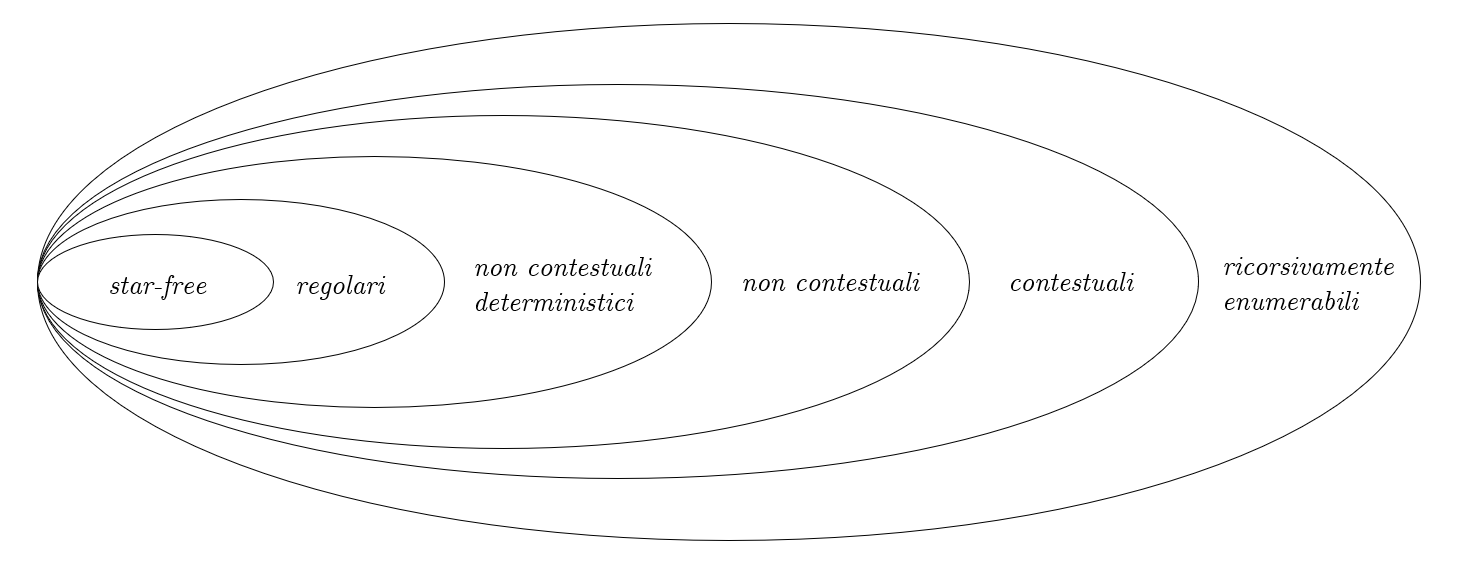
\includegraphics[width=17cm]{gerarchia linguaggi.png} 
  \caption{Gerarchia dei linguaggi}
\end{figure}

\break

\section{Logica per la descrizione di Proprietà}
Quando si programma una funzione è importante definire con precisione quale sia il suo funzionamento, senza necessariamente descrivere come funzioni. A tal proposito si è soliti scrivere le cosiddette prcondizioni e postcondizioni:
\begin{itemize}
  \item Precondizione: indica le condizioni che devono valere prima che la funzione venga invocata;
  \item Postcondizione: indica le condizioni che devono valere al termine dell'esecuzione del programma.  
\end{itemize}

Dunque, il programma \(P\) deve essere tale per cui se la precondizione \(Pre\) vale prima dell'esecuzione di tale programma, allora la post condizione \(Post\) deve valere dopo l'esecuzione. Tali condizioni possono essere espresse in linguaggi diversi, ma il più comune è la logica del primo ordine.